% Options for packages loaded elsewhere
\PassOptionsToPackage{unicode}{hyperref}
\PassOptionsToPackage{hyphens}{url}
%
\documentclass[
]{article}
\usepackage{lmodern}
\usepackage{amssymb,amsmath}
\usepackage{ifxetex,ifluatex}
\ifnum 0\ifxetex 1\fi\ifluatex 1\fi=0 % if pdftex
  \usepackage[T1]{fontenc}
  \usepackage[utf8]{inputenc}
  \usepackage{textcomp} % provide euro and other symbols
\else % if luatex or xetex
  \usepackage{unicode-math}
  \defaultfontfeatures{Scale=MatchLowercase}
  \defaultfontfeatures[\rmfamily]{Ligatures=TeX,Scale=1}
\fi
% Use upquote if available, for straight quotes in verbatim environments
\IfFileExists{upquote.sty}{\usepackage{upquote}}{}
\IfFileExists{microtype.sty}{% use microtype if available
  \usepackage[]{microtype}
  \UseMicrotypeSet[protrusion]{basicmath} % disable protrusion for tt fonts
}{}
\makeatletter
\@ifundefined{KOMAClassName}{% if non-KOMA class
  \IfFileExists{parskip.sty}{%
    \usepackage{parskip}
  }{% else
    \setlength{\parindent}{0pt}
    \setlength{\parskip}{6pt plus 2pt minus 1pt}}
}{% if KOMA class
  \KOMAoptions{parskip=half}}
\makeatother
\usepackage{xcolor}
\IfFileExists{xurl.sty}{\usepackage{xurl}}{} % add URL line breaks if available
\IfFileExists{bookmark.sty}{\usepackage{bookmark}}{\usepackage{hyperref}}
\hypersetup{
  pdftitle={Flujo de análisis en clasificación supervisada},
  pdfauthor={Laura Rodríguez Navas},
  hidelinks,
  pdfcreator={LaTeX via pandoc}}
\urlstyle{same} % disable monospaced font for URLs
\usepackage[margin=1in]{geometry}
\usepackage{color}
\usepackage{fancyvrb}
\newcommand{\VerbBar}{|}
\newcommand{\VERB}{\Verb[commandchars=\\\{\}]}
\DefineVerbatimEnvironment{Highlighting}{Verbatim}{commandchars=\\\{\}}
% Add ',fontsize=\small' for more characters per line
\usepackage{framed}
\definecolor{shadecolor}{RGB}{248,248,248}
\newenvironment{Shaded}{\begin{snugshade}}{\end{snugshade}}
\newcommand{\AlertTok}[1]{\textcolor[rgb]{0.94,0.16,0.16}{#1}}
\newcommand{\AnnotationTok}[1]{\textcolor[rgb]{0.56,0.35,0.01}{\textbf{\textit{#1}}}}
\newcommand{\AttributeTok}[1]{\textcolor[rgb]{0.77,0.63,0.00}{#1}}
\newcommand{\BaseNTok}[1]{\textcolor[rgb]{0.00,0.00,0.81}{#1}}
\newcommand{\BuiltInTok}[1]{#1}
\newcommand{\CharTok}[1]{\textcolor[rgb]{0.31,0.60,0.02}{#1}}
\newcommand{\CommentTok}[1]{\textcolor[rgb]{0.56,0.35,0.01}{\textit{#1}}}
\newcommand{\CommentVarTok}[1]{\textcolor[rgb]{0.56,0.35,0.01}{\textbf{\textit{#1}}}}
\newcommand{\ConstantTok}[1]{\textcolor[rgb]{0.00,0.00,0.00}{#1}}
\newcommand{\ControlFlowTok}[1]{\textcolor[rgb]{0.13,0.29,0.53}{\textbf{#1}}}
\newcommand{\DataTypeTok}[1]{\textcolor[rgb]{0.13,0.29,0.53}{#1}}
\newcommand{\DecValTok}[1]{\textcolor[rgb]{0.00,0.00,0.81}{#1}}
\newcommand{\DocumentationTok}[1]{\textcolor[rgb]{0.56,0.35,0.01}{\textbf{\textit{#1}}}}
\newcommand{\ErrorTok}[1]{\textcolor[rgb]{0.64,0.00,0.00}{\textbf{#1}}}
\newcommand{\ExtensionTok}[1]{#1}
\newcommand{\FloatTok}[1]{\textcolor[rgb]{0.00,0.00,0.81}{#1}}
\newcommand{\FunctionTok}[1]{\textcolor[rgb]{0.00,0.00,0.00}{#1}}
\newcommand{\ImportTok}[1]{#1}
\newcommand{\InformationTok}[1]{\textcolor[rgb]{0.56,0.35,0.01}{\textbf{\textit{#1}}}}
\newcommand{\KeywordTok}[1]{\textcolor[rgb]{0.13,0.29,0.53}{\textbf{#1}}}
\newcommand{\NormalTok}[1]{#1}
\newcommand{\OperatorTok}[1]{\textcolor[rgb]{0.81,0.36,0.00}{\textbf{#1}}}
\newcommand{\OtherTok}[1]{\textcolor[rgb]{0.56,0.35,0.01}{#1}}
\newcommand{\PreprocessorTok}[1]{\textcolor[rgb]{0.56,0.35,0.01}{\textit{#1}}}
\newcommand{\RegionMarkerTok}[1]{#1}
\newcommand{\SpecialCharTok}[1]{\textcolor[rgb]{0.00,0.00,0.00}{#1}}
\newcommand{\SpecialStringTok}[1]{\textcolor[rgb]{0.31,0.60,0.02}{#1}}
\newcommand{\StringTok}[1]{\textcolor[rgb]{0.31,0.60,0.02}{#1}}
\newcommand{\VariableTok}[1]{\textcolor[rgb]{0.00,0.00,0.00}{#1}}
\newcommand{\VerbatimStringTok}[1]{\textcolor[rgb]{0.31,0.60,0.02}{#1}}
\newcommand{\WarningTok}[1]{\textcolor[rgb]{0.56,0.35,0.01}{\textbf{\textit{#1}}}}
\usepackage{graphicx,grffile}
\makeatletter
\def\maxwidth{\ifdim\Gin@nat@width>\linewidth\linewidth\else\Gin@nat@width\fi}
\def\maxheight{\ifdim\Gin@nat@height>\textheight\textheight\else\Gin@nat@height\fi}
\makeatother
% Scale images if necessary, so that they will not overflow the page
% margins by default, and it is still possible to overwrite the defaults
% using explicit options in \includegraphics[width, height, ...]{}
\setkeys{Gin}{width=\maxwidth,height=\maxheight,keepaspectratio}
% Set default figure placement to htbp
\makeatletter
\def\fps@figure{htbp}
\makeatother
\setlength{\emergencystretch}{3em} % prevent overfull lines
\providecommand{\tightlist}{%
  \setlength{\itemsep}{0pt}\setlength{\parskip}{0pt}}
\setcounter{secnumdepth}{5}

\title{Flujo de análisis en clasificación supervisada}
\usepackage{etoolbox}
\makeatletter
\providecommand{\subtitle}[1]{% add subtitle to \maketitle
  \apptocmd{\@title}{\par {\large #1 \par}}{}{}
}
\makeatother
\subtitle{Métodos supervisados}
\author{Laura Rodríguez Navas}
\date{Septiembre 2020}

\begin{document}
\maketitle

{
\setcounter{tocdepth}{2}
\tableofcontents
}
Comenzamos cargando los paquetes y la base de datos:

\begin{Shaded}
\begin{Highlighting}[]
\KeywordTok{library}\NormalTok{(caret)}
\KeywordTok{library}\NormalTok{(mlbench)}
\KeywordTok{data}\NormalTok{(Sonar)}
\KeywordTok{str}\NormalTok{(Sonar, }\DataTypeTok{width =} \DecValTok{85}\NormalTok{, }\DataTypeTok{strict.width =} \StringTok{"cut"}\NormalTok{)}
\end{Highlighting}
\end{Shaded}

\begin{verbatim}
## 'data.frame':    208 obs. of  61 variables:
##  $ V1   : num  0.02 0.0453 0.0262 0.01 0.0762 0.0286 0.0317 0.0519 0.0223 0.0164 ...
##  $ V2   : num  0.0371 0.0523 0.0582 0.0171 0.0666 0.0453 0.0956 0.0548 0.0375 0.017..
##  $ V3   : num  0.0428 0.0843 0.1099 0.0623 0.0481 ...
##  $ V4   : num  0.0207 0.0689 0.1083 0.0205 0.0394 ...
##  $ V5   : num  0.0954 0.1183 0.0974 0.0205 0.059 ...
##  $ V6   : num  0.0986 0.2583 0.228 0.0368 0.0649 ...
##  $ V7   : num  0.154 0.216 0.243 0.11 0.121 ...
##  $ V8   : num  0.16 0.348 0.377 0.128 0.247 ...
##  $ V9   : num  0.3109 0.3337 0.5598 0.0598 0.3564 ...
##  $ V10  : num  0.211 0.287 0.619 0.126 0.446 ...
##  $ V11  : num  0.1609 0.4918 0.6333 0.0881 0.4152 ...
##  $ V12  : num  0.158 0.655 0.706 0.199 0.395 ...
##  $ V13  : num  0.2238 0.6919 0.5544 0.0184 0.4256 ...
##  $ V14  : num  0.0645 0.7797 0.532 0.2261 0.4135 ...
##  $ V15  : num  0.066 0.746 0.648 0.173 0.453 ...
##  $ V16  : num  0.227 0.944 0.693 0.213 0.533 ...
##  $ V17  : num  0.31 1 0.6759 0.0693 0.7306 ...
##  $ V18  : num  0.3 0.887 0.755 0.228 0.619 ...
##  $ V19  : num  0.508 0.802 0.893 0.406 0.203 ...
##  $ V20  : num  0.48 0.782 0.862 0.397 0.464 ...
##  $ V21  : num  0.578 0.521 0.797 0.274 0.415 ...
##  $ V22  : num  0.507 0.405 0.674 0.369 0.429 ...
##  $ V23  : num  0.433 0.396 0.429 0.556 0.573 ...
##  $ V24  : num  0.555 0.391 0.365 0.485 0.54 ...
##  $ V25  : num  0.671 0.325 0.533 0.314 0.316 ...
##  $ V26  : num  0.641 0.32 0.241 0.533 0.229 ...
##  $ V27  : num  0.71 0.327 0.507 0.526 0.7 ...
##  $ V28  : num  0.808 0.277 0.853 0.252 1 ...
##  $ V29  : num  0.679 0.442 0.604 0.209 0.726 ...
##  $ V30  : num  0.386 0.203 0.851 0.356 0.472 ...
##  $ V31  : num  0.131 0.379 0.851 0.626 0.51 ...
##  $ V32  : num  0.26 0.295 0.504 0.734 0.546 ...
##  $ V33  : num  0.512 0.198 0.186 0.612 0.288 ...
##  $ V34  : num  0.7547 0.2341 0.2709 0.3497 0.0981 ...
##  $ V35  : num  0.854 0.131 0.423 0.395 0.195 ...
##  $ V36  : num  0.851 0.418 0.304 0.301 0.418 ...
##  $ V37  : num  0.669 0.384 0.612 0.541 0.46 ...
##  $ V38  : num  0.61 0.106 0.676 0.881 0.322 ...
##  $ V39  : num  0.494 0.184 0.537 0.986 0.283 ...
##  $ V40  : num  0.274 0.197 0.472 0.917 0.243 ...
##  $ V41  : num  0.051 0.167 0.465 0.612 0.198 ...
##  $ V42  : num  0.2834 0.0583 0.2587 0.5006 0.2444 ...
##  $ V43  : num  0.282 0.14 0.213 0.321 0.185 ...
##  $ V44  : num  0.4256 0.1628 0.2222 0.3202 0.0841 ...
##  $ V45  : num  0.2641 0.0621 0.2111 0.4295 0.0692 ...
##  $ V46  : num  0.1386 0.0203 0.0176 0.3654 0.0528 ...
##  $ V47  : num  0.1051 0.053 0.1348 0.2655 0.0357 ...
##  $ V48  : num  0.1343 0.0742 0.0744 0.1576 0.0085 ...
##  $ V49  : num  0.0383 0.0409 0.013 0.0681 0.023 0.0264 0.0507 0.0285 0.0777 0.0092 ..
##  $ V50  : num  0.0324 0.0061 0.0106 0.0294 0.0046 0.0081 0.0159 0.0178 0.0439 0.019..
##  $ V51  : num  0.0232 0.0125 0.0033 0.0241 0.0156 0.0104 0.0195 0.0052 0.0061 0.011..
##  $ V52  : num  0.0027 0.0084 0.0232 0.0121 0.0031 0.0045 0.0201 0.0081 0.0145 0.009..
##  $ V53  : num  0.0065 0.0089 0.0166 0.0036 0.0054 0.0014 0.0248 0.012 0.0128 0.0223..
##  $ V54  : num  0.0159 0.0048 0.0095 0.015 0.0105 0.0038 0.0131 0.0045 0.0145 0.0179..
##  $ V55  : num  0.0072 0.0094 0.018 0.0085 0.011 0.0013 0.007 0.0121 0.0058 0.0084 ...
##  $ V56  : num  0.0167 0.0191 0.0244 0.0073 0.0015 0.0089 0.0138 0.0097 0.0049 0.006..
##  $ V57  : num  0.018 0.014 0.0316 0.005 0.0072 0.0057 0.0092 0.0085 0.0065 0.0032 ...
##  $ V58  : num  0.0084 0.0049 0.0164 0.0044 0.0048 0.0027 0.0143 0.0047 0.0093 0.003..
##  $ V59  : num  0.009 0.0052 0.0095 0.004 0.0107 0.0051 0.0036 0.0048 0.0059 0.0056 ..
##  $ V60  : num  0.0032 0.0044 0.0078 0.0117 0.0094 0.0062 0.0103 0.0053 0.0022 0.004..
##  $ Class: Factor w/ 2 levels "M","R": 2 2 2 2 2 2 2 2 2 2 ...
\end{verbatim}

\hypertarget{ejercicio-propuesto}{%
\subsection{Ejercicio propuesto}\label{ejercicio-propuesto}}

Cargamos las librerías necesarias:

\begin{Shaded}
\begin{Highlighting}[]
\KeywordTok{library}\NormalTok{(tidyverse)}
\KeywordTok{library}\NormalTok{(tm)}
\KeywordTok{library}\NormalTok{(SnowballC)}
\end{Highlighting}
\end{Shaded}

El dataset escogido se puede encontrar en
(\url{https://www.kaggle.com/c/nlp-getting-started/data}). Este dataset,
con 10.876 instancias, contiene 4 variables explicativas; \emph{id},
\emph{keyword}, \emph{location} y \emph{test}, y dos valores en la
variable clase \emph{target} (1 y 0). La variable clase es de tipo
binaria así que vamos a aprender un modelo de clasificación binaria, y
vamos a predecir si dado un tweet, este tweet trata sobre un desastre
real o no. Si es un desastre real, se predice un 1. Si no, se predice un
0.

La partición inicial train-test, no se tiene que realizar, ya que las
instancias de train y test ya vienen definidas en los ficheros
\emph{train.csv} y \emph{test.csv}, proporcionados por la competición en
\href{https://www.kaggle.com/c/nlp-getting-started/overview}{Kaggle} que
se ha elegido. El conjunto de datos de train contiene 7613 instancias y
el conjunto de datos de test contiene 3262 instancias.

Cargamos el dataset:

\begin{Shaded}
\begin{Highlighting}[]
\NormalTok{train <-}\StringTok{ }\KeywordTok{read.csv}\NormalTok{(}\StringTok{"train.csv"}\NormalTok{, }\DataTypeTok{na.strings=}\KeywordTok{c}\NormalTok{(}\StringTok{""}\NormalTok{,}\StringTok{"NA"}\NormalTok{))}
\KeywordTok{dim}\NormalTok{(train)}
\end{Highlighting}
\end{Shaded}

\begin{verbatim}
## [1] 7613    5
\end{verbatim}

\begin{Shaded}
\begin{Highlighting}[]
\NormalTok{test <-}\StringTok{ }\KeywordTok{read.csv}\NormalTok{(}\StringTok{"test.csv"}\NormalTok{, }\DataTypeTok{na.strings=}\KeywordTok{c}\NormalTok{(}\StringTok{""}\NormalTok{,}\StringTok{"NA"}\NormalTok{))}
\KeywordTok{dim}\NormalTok{(test)}
\end{Highlighting}
\end{Shaded}

\begin{verbatim}
## [1] 3263    4
\end{verbatim}

Cada instancia en el conjunto de train y test contiene la siguiente
información:

\begin{itemize}
\tightlist
\item
  \textbf{id}: un identificador único para cada tweet.
\item
  \textbf{keyword}: una palabra clave del tweet (puede estar en blanco).
\item
  \textbf{location}: la ubicación desde la que se envió el tweet (puede
  estar en blanco).
\item
  \textbf{text}: el texto del tweet.
\item
  \textbf{target}: solo en el conjunto de datos de train porqué es la
  variable clase a predecir. Indica si un tweet es sobre un desastre
  real (1) o no (0).
\end{itemize}

\begin{Shaded}
\begin{Highlighting}[]
\KeywordTok{str}\NormalTok{(train)}
\end{Highlighting}
\end{Shaded}

\begin{verbatim}
## 'data.frame':    7613 obs. of  5 variables:
##  $ id      : int  1 4 5 6 7 8 10 13 14 15 ...
##  $ keyword : chr  NA NA NA NA ...
##  $ location: chr  NA NA NA NA ...
##  $ text    : chr  "Our Deeds are the Reason of this #earthquake May ALLAH Forgive us all" "Forest fire near La Ronge Sask. Canada" "All residents asked to 'shelter in place' are being notified by officers. No other evacuation or shelter in pla"| __truncated__ "13,000 people receive #wildfires evacuation orders in California " ...
##  $ target  : int  1 1 1 1 1 1 1 1 1 1 ...
\end{verbatim}

\begin{Shaded}
\begin{Highlighting}[]
\KeywordTok{str}\NormalTok{(test)}
\end{Highlighting}
\end{Shaded}

\begin{verbatim}
## 'data.frame':    3263 obs. of  4 variables:
##  $ id      : int  0 2 3 9 11 12 21 22 27 29 ...
##  $ keyword : chr  NA NA NA NA ...
##  $ location: chr  NA NA NA NA ...
##  $ text    : chr  "Just happened a terrible car crash" "Heard about #earthquake is different cities, stay safe everyone." "there is a forest fire at spot pond, geese are fleeing across the street, I cannot save them all" "Apocalypse lighting. #Spokane #wildfires" ...
\end{verbatim}

Factorización de la variable clase, que inicialmente es de tipo entero.

\begin{Shaded}
\begin{Highlighting}[]
\KeywordTok{str}\NormalTok{(train}\OperatorTok{$}\NormalTok{target)}
\end{Highlighting}
\end{Shaded}

\begin{verbatim}
##  int [1:7613] 1 1 1 1 1 1 1 1 1 1 ...
\end{verbatim}

\begin{Shaded}
\begin{Highlighting}[]
\NormalTok{train}\OperatorTok{$}\NormalTok{target <-}\StringTok{ }\KeywordTok{as.factor}\NormalTok{(train}\OperatorTok{$}\NormalTok{target)}
\KeywordTok{str}\NormalTok{(train}\OperatorTok{$}\NormalTok{target)}
\end{Highlighting}
\end{Shaded}

\begin{verbatim}
##  Factor w/ 2 levels "0","1": 2 2 2 2 2 2 2 2 2 2 ...
\end{verbatim}

Distribución de la variable clase:

\begin{Shaded}
\begin{Highlighting}[]
\KeywordTok{ggplot}\NormalTok{(train, }\KeywordTok{aes}\NormalTok{(}\DataTypeTok{x=}\NormalTok{target)) }\OperatorTok{+}\StringTok{ }
\StringTok{  }\KeywordTok{geom_bar}\NormalTok{(}\KeywordTok{aes}\NormalTok{(}\DataTypeTok{fill=}\NormalTok{target))}
\end{Highlighting}
\end{Shaded}

\begin{center}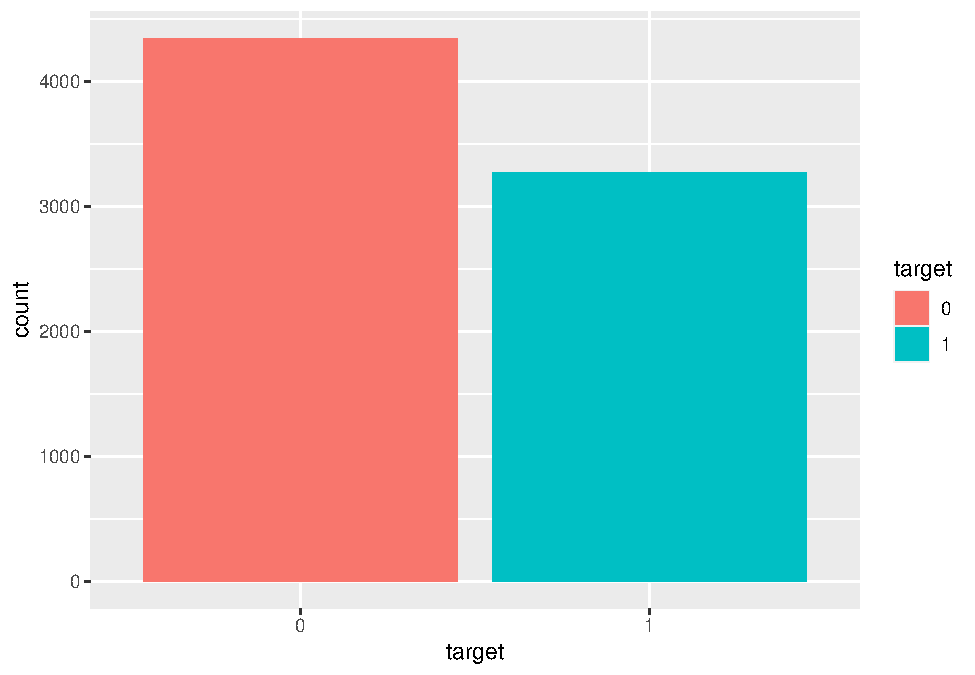
\includegraphics{exercise_files/figure-latex/unnamed-chunk-6-1} \end{center}

\begin{Shaded}
\begin{Highlighting}[]
\KeywordTok{sum}\NormalTok{(train}\OperatorTok{$}\NormalTok{target }\OperatorTok{==}\StringTok{ "0"}\NormalTok{) }\OperatorTok{/}\StringTok{ }\KeywordTok{dim}\NormalTok{(train)[}\DecValTok{1}\NormalTok{] }\OperatorTok{*}\StringTok{ }\DecValTok{100}
\end{Highlighting}
\end{Shaded}

\begin{verbatim}
## [1] 57.03402
\end{verbatim}

\begin{Shaded}
\begin{Highlighting}[]
\KeywordTok{sum}\NormalTok{(train}\OperatorTok{$}\NormalTok{target }\OperatorTok{==}\StringTok{ "1"}\NormalTok{) }\OperatorTok{/}\StringTok{ }\KeywordTok{dim}\NormalTok{(train)[}\DecValTok{1}\NormalTok{] }\OperatorTok{*}\StringTok{ }\DecValTok{100}
\end{Highlighting}
\end{Shaded}

\begin{verbatim}
## [1] 42.96598
\end{verbatim}

La distribución de la variable a predecir está relativamente
equilibrada, donde el 57\% de las instancias de los tweets son sobre un
desastre no real y el 43\% sobre un desastre real.

\hypertarget{correlaciones-entre-variables-explicativas}{%
\subsubsection{correlaciones entre variables
explicativas}\label{correlaciones-entre-variables-explicativas}}

\hypertarget{muxe9tica-de-evaluaciuxf3n}{%
\subsubsection{mética de evaluación}\label{muxe9tica-de-evaluaciuxf3n}}

\hypertarget{valores-perdidos}{%
\subsubsection{valores perdidos}\label{valores-perdidos}}

\begin{Shaded}
\begin{Highlighting}[]
\KeywordTok{colSums}\NormalTok{(}\KeywordTok{sapply}\NormalTok{(train, is.na))}
\end{Highlighting}
\end{Shaded}

\begin{verbatim}
##       id  keyword location     text   target 
##        0       61     2533        0        0
\end{verbatim}

\begin{Shaded}
\begin{Highlighting}[]
\KeywordTok{colSums}\NormalTok{(}\KeywordTok{sapply}\NormalTok{(test, is.na))}
\end{Highlighting}
\end{Shaded}

\begin{verbatim}
##       id  keyword location     text 
##        0       26     1105        0
\end{verbatim}

Las variables \emph{keyword} y \emph{location} tienen valores perdidos.
Sobretodo hay una gran cantidad de tweets, para los cuales falta la
ubicación. Potencialmente, esto podría ser una buena variable predictiva
en sí misma. No faltan valores en las variables \emph{target} y
\emph{text}.

Nos ocuparemos de los valores perdidos más adelante.

Eliminamos la variable \emph{id}.

\begin{Shaded}
\begin{Highlighting}[]
\NormalTok{train}\OperatorTok{$}\NormalTok{id <-}\StringTok{ }\OtherTok{NULL}
\NormalTok{test}\OperatorTok{$}\NormalTok{id <-}\StringTok{ }\OtherTok{NULL}
\end{Highlighting}
\end{Shaded}

\hypertarget{keyword}{%
\subsection{keyword}\label{keyword}}

\begin{Shaded}
\begin{Highlighting}[]
\KeywordTok{length}\NormalTok{(}\KeywordTok{unique}\NormalTok{(train}\OperatorTok{$}\NormalTok{keyword))}
\end{Highlighting}
\end{Shaded}

\begin{verbatim}
## [1] 222
\end{verbatim}

\begin{Shaded}
\begin{Highlighting}[]
\KeywordTok{length}\NormalTok{(}\KeywordTok{unique}\NormalTok{(test}\OperatorTok{$}\NormalTok{keyword))}
\end{Highlighting}
\end{Shaded}

\begin{verbatim}
## [1] 222
\end{verbatim}

\begin{Shaded}
\begin{Highlighting}[]
\NormalTok{train}\OperatorTok{$}\NormalTok{keyword <-}\StringTok{ }\KeywordTok{as.factor}\NormalTok{(train}\OperatorTok{$}\NormalTok{keyword)}
\KeywordTok{all.equal}\NormalTok{(}\KeywordTok{levels}\NormalTok{(train}\OperatorTok{$}\NormalTok{keyword), }\KeywordTok{levels}\NormalTok{(test}\OperatorTok{$}\NormalTok{keyword))}
\end{Highlighting}
\end{Shaded}

\begin{verbatim}
## [1] "Modes: character, NULL"              
## [2] "Lengths: 221, 0"                     
## [3] "target is character, current is NULL"
\end{verbatim}

\hypertarget{location}{%
\subsection{location}\label{location}}

\begin{Shaded}
\begin{Highlighting}[]
\KeywordTok{length}\NormalTok{(}\KeywordTok{unique}\NormalTok{(train}\OperatorTok{$}\NormalTok{location))}
\end{Highlighting}
\end{Shaded}

\begin{verbatim}
## [1] 3342
\end{verbatim}

\begin{Shaded}
\begin{Highlighting}[]
\KeywordTok{length}\NormalTok{(}\KeywordTok{unique}\NormalTok{(test}\OperatorTok{$}\NormalTok{location))}
\end{Highlighting}
\end{Shaded}

\begin{verbatim}
## [1] 1603
\end{verbatim}

\begin{Shaded}
\begin{Highlighting}[]
\NormalTok{train_and_test <-}\StringTok{ }\KeywordTok{rbind}\NormalTok{(train[, }\DecValTok{1}\OperatorTok{:}\DecValTok{3}\NormalTok{], test)}
\KeywordTok{str}\NormalTok{(train_and_test)}
\end{Highlighting}
\end{Shaded}

\begin{verbatim}
## 'data.frame':    10876 obs. of  3 variables:
##  $ keyword : Factor w/ 221 levels "ablaze","accident",..: NA NA NA NA NA NA NA NA NA NA ...
##  $ location: chr  NA NA NA NA ...
##  $ text    : chr  "Our Deeds are the Reason of this #earthquake May ALLAH Forgive us all" "Forest fire near La Ronge Sask. Canada" "All residents asked to 'shelter in place' are being notified by officers. No other evacuation or shelter in pla"| __truncated__ "13,000 people receive #wildfires evacuation orders in California " ...
\end{verbatim}

\begin{enumerate}
\def\labelenumi{\arabic{enumi}.}
\tightlist
\item
  Create a corpus
\item
  Convert to lowercase
\item
  Remove punctuation
\item
  Remove stopwords
\item
  Stemming (using Porter's stemming algorithm)
\item
  Create document term matrix
\end{enumerate}

\begin{Shaded}
\begin{Highlighting}[]
\NormalTok{corpus_location <-}\StringTok{ }\KeywordTok{Corpus}\NormalTok{(}\KeywordTok{VectorSource}\NormalTok{(train_and_test}\OperatorTok{$}\NormalTok{location))}
\NormalTok{corpus_location[[}\DecValTok{33}\NormalTok{]]}\OperatorTok{$}\NormalTok{content}
\end{Highlighting}
\end{Shaded}

\begin{verbatim}
## [1] "Est. September 2012 - Bristol"
\end{verbatim}

\begin{Shaded}
\begin{Highlighting}[]
\NormalTok{corpus_location <-}\StringTok{ }\KeywordTok{tm_map}\NormalTok{(corpus_location, tolower)}
\NormalTok{corpus_location[[}\DecValTok{33}\NormalTok{]]}\OperatorTok{$}\NormalTok{content}
\end{Highlighting}
\end{Shaded}

\begin{verbatim}
## [1] "est. september 2012 - bristol"
\end{verbatim}

\begin{Shaded}
\begin{Highlighting}[]
\NormalTok{corpus_location <-}\StringTok{ }\KeywordTok{tm_map}\NormalTok{(corpus_location, removePunctuation)}
\NormalTok{corpus_location[[}\DecValTok{33}\NormalTok{]]}\OperatorTok{$}\NormalTok{content}
\end{Highlighting}
\end{Shaded}

\begin{verbatim}
## [1] "est september 2012  bristol"
\end{verbatim}

\begin{Shaded}
\begin{Highlighting}[]
\NormalTok{corpus_location <-}\StringTok{ }\KeywordTok{tm_map}\NormalTok{(corpus_location, removeWords, }\KeywordTok{stopwords}\NormalTok{(}\StringTok{"english"}\NormalTok{))}
\NormalTok{corpus_location[[}\DecValTok{33}\NormalTok{]]}\OperatorTok{$}\NormalTok{content}
\end{Highlighting}
\end{Shaded}

\begin{verbatim}
## [1] "est september 2012  bristol"
\end{verbatim}

\begin{Shaded}
\begin{Highlighting}[]
\NormalTok{corpus_location <-}\StringTok{ }\KeywordTok{tm_map}\NormalTok{(corpus_location, stemDocument)}
\NormalTok{corpus_location[[}\DecValTok{33}\NormalTok{]]}\OperatorTok{$}\NormalTok{content}
\end{Highlighting}
\end{Shaded}

\begin{verbatim}
## [1] "est septemb 2012 bristol"
\end{verbatim}

\begin{itemize}
\tightlist
\item
  Create document term matrix
\item
  Reduce sparsity
\item
  Convert to data frame
\end{itemize}

\begin{Shaded}
\begin{Highlighting}[]
\NormalTok{dtm_location <-}\StringTok{ }\KeywordTok{DocumentTermMatrix}\NormalTok{(corpus_location)}
\NormalTok{dtm_location}
\end{Highlighting}
\end{Shaded}

\begin{verbatim}
## <<DocumentTermMatrix (documents: 10876, terms: 3840)>>
## Non-/sparse entries: 11855/41751985
## Sparsity           : 100%
## Maximal term length: 41
## Weighting          : term frequency (tf)
\end{verbatim}

\begin{Shaded}
\begin{Highlighting}[]
\NormalTok{dtm_location <-}\StringTok{ }\KeywordTok{removeSparseTerms}\NormalTok{(dtm_location, }\FloatTok{0.9975}\NormalTok{)}
\NormalTok{dtm_location}
\end{Highlighting}
\end{Shaded}

\begin{verbatim}
## <<DocumentTermMatrix (documents: 10876, terms: 55)>>
## Non-/sparse entries: 3967/594213
## Sparsity           : 99%
## Maximal term length: 10
## Weighting          : term frequency (tf)
\end{verbatim}

\begin{Shaded}
\begin{Highlighting}[]
\NormalTok{bag_of_words_location <-}\StringTok{ }\KeywordTok{as.data.frame}\NormalTok{(}\KeywordTok{as.matrix}\NormalTok{(dtm_location))}
\KeywordTok{colnames}\NormalTok{(bag_of_words_location) <-}\StringTok{ }\KeywordTok{paste0}\NormalTok{(}\KeywordTok{colnames}\NormalTok{(bag_of_words_location), }\StringTok{"_location"}\NormalTok{)}
\KeywordTok{str}\NormalTok{(bag_of_words_location, }\DataTypeTok{list.len=}\DecValTok{10}\NormalTok{)}
\end{Highlighting}
\end{Shaded}

\begin{verbatim}
## 'data.frame':    10876 obs. of  55 variables:
##  $ africa_location    : num  0 0 0 0 0 0 0 0 0 0 ...
##  $ london_location    : num  0 0 0 0 0 0 0 0 0 0 ...
##  $ world_location     : num  0 0 0 0 0 0 0 0 0 0 ...
##  $ citi_location      : num  0 0 0 0 0 0 0 0 0 0 ...
##  $ carolina_location  : num  0 0 0 0 0 0 0 0 0 0 ...
##  $ england_location   : num  0 0 0 0 0 0 0 0 0 0 ...
##  $ ohio_location      : num  0 0 0 0 0 0 0 0 0 0 ...
##  $ india_location     : num  0 0 0 0 0 0 0 0 0 0 ...
##  $ usa_location       : num  0 0 0 0 0 0 0 0 0 0 ...
##  $ south_location     : num  0 0 0 0 0 0 0 0 0 0 ...
##   [list output truncated]
\end{verbatim}

\hypertarget{text}{%
\subsection{text}\label{text}}

\end{document}
